%!TEX root = ../main.tex

\section{Evaluation}
We run experiments on a Linux machine with 80 CPU cores, 500GB RAM, and 2 GPUs. To evaluate Qsearch, we perform an intrinsic evaluation of our {\em Qfact extraction model} and an extrinsic evaluation of the {\em end-to-end Qsearch system}.
\subsubsection{Dataset.} All experiments use a large collection of news articles, compiled from two real world datasets: the \textit{STICS} project \cite{DBLP:conf/sigir/HoffartMW14} with news from 2014 to 2018, 
and the \textit{New York Times} archive
\cite{nyt}
 %5843811 + 1765538
with news from 1986 to 2008.
In total, our corpus consists of 7.6M documents.
 
\subsection{Intrinsic Evaluation of the Quantity Fact Extraction Model}
%We conduct intrinsic evaluation to examine the quality of our Qfact extraction model of the %\textit{Extract} stage.
\subsubsection{Training setup.}
We implemented the  LSTM network using Theano library,
largely following \cite{DBLP:conf/acl/HeLLZ17a} for the training 
configuration: using Adadelta with $\epsilon = 1e^6$ and $\rho = 0.95$;  \textit{lstm\_hidden\_unit = 300}; \textit{rnn\_dropout\_prob = 0.1}; \textit{batch\_size = 100}.

We extracted training samples from the corpus using the distant-supervision technique as described in Section \ref{sec:extract} and conducted the training process with different settings. 
In the \textit{General} setting, we use all available training data
of 3.2M training samples, where we maintain the ratio 3:1 between the number of positive and negative samples.
We also train our model for three other 
\textit{measure-specific} settings, where only a subset of the training samples is used. In particular, we classify training samples into different categories based on the quantity unit. For example, training samples containing quantities with unit \textit{Kilometer} or \textit{Meter} are chosen to train the model in the \textit{Length} setting, while the ones with unit \textit{US dollar}, \textit{Euro}, etc. are picked for the \textit{Money} setting. 
Among many such categories, we selected the three most prevalent measures \textit{Money}, \textit{Percentage} and \textit{Length}, containing 307K, 235K and 41K training samples, respectively (also with ratio 3:1  between positive and negative samples). 
%to train the corresponding models. 
The trained models are then applied to the entire corpus to extract more Qfacts. 
%Note that the input for the trained models should be compatible with their trained settings.

\subsubsection{Performance of Extraction model.}
As the test data does not have any ground-truth labels, 
we randomly selected 100 samples that contain at least two entities from the output tag sequences, for each training model, and manually assessed their validity.
\begin{table}[t]
\centering
\caption{Evaluation of Qfact extraction model of Qsearch on different settings.}
\begin{tabular}{c |r r r|r r r|r r r|r r r} \midrule
 \multirow{2}{*}{\textbf{Tag}} & \multicolumn{3}{c}{\textbf{Length}} & \multicolumn{3}{|c}{\textbf{Money}}  & \multicolumn{3}{|c}{\textbf{Percentage}}  & \multicolumn{3}{|c}{\textbf{General}} \\
 \cmidrule{2-13}
 & \textit{~Prec.} &  \textit{~~~Rec.} & \textit{~~~~~F1~} & \textit{~Prec.} &  \textit{~~~Rec.} & \textit{~~~~~F1~} & \textit{~Prec.} &  \textit{~~~Rec.} & \textit{~~~~~F1~} & \textit{~Prec.} &  \textit{~~~Rec.} & \textit{~~~~~F1~} \\
 \midrule
\textbf{E} & 0.860 & 0.860 & 0.860 & 0.850 & 0.850 & 0.850 & 0.794 & 0.770 & 0.782 & 0.882 & 0.820 & 0.850 \\
\textbf{X} & 0.650 & 0.849 & 0.736 & 0.717 & 0.844 & 0.776 & 0.659 & 0.827 & 0.734 & 0.728 & 0.713 & 0.721 \\
\textbf{O} & 0.958 & 0.886 & 0.920 & 0.942 & 0.886 & 0.913 & 0.947 & 0.888 & 0.917 & 0.895 & 0.906 & 0.900 \\
 \midrule
\textbf{Macro-avg.} & 0.823 & 0.865 & 0.839 & 0.836 & 0.860 & 0.846 & 0.800 & 0.828 & 0.811 & 0.835 & 0.813 & 0.824 \\
 \midrule
\end{tabular}
\label{table:extract_quality}
\end{table}

We evaluate the quality of the three output labels \textit{<E>}, \textit{<X>} and \textit{<O>} by three measures: \textit{Precision}, \textit{Recall}, and \textit{F1 score}.
The results are shown in Table \ref{table:extract_quality}. 
We observe that all training models perform very well on entity tagging with more than 85\% \textit{F1 score}. 
%This assures that our model can efficiently identify the referred entity for a given quantity. 
%The results also show that the extraction models can capture around 70\% of correct context %tokens of the Qfacts.
We also see that the measure-specific training variants for Length and Money
have slight advantages.

%Moreover, the extraction model also achieves at least 90\% accuracy in identifying \textit{<O>} tag, which helps to reduce the noisy candidates for answer generation step. 

%%%%%%%%%%%%%%%%%%%%%%%%%%%%%%%%%%%%%%%

\subsection{Extrinsic Evaluation of the End-to-End Qsearch System}
We performed the extrinsic evaluation of Qsearch 
on a benchmark of 100  quantity queries, collected by crowdsourcing
and covering four domains: \textit{Finance}, \textit{Transport}, \textit{Sports} and \textit{Technology}. 
These queries capture a wide diversity of measures and units as well as variety in query formulations
(e.g., phrases for the comparison operators); see Table~\ref{table:query_stat}. 
%Conditional phrases are also varies widely, e.g., less than, above, over, etc. 
Anecdotal examples of user queries and their answers produced by Qsearch are shown in Table~\ref{table:example_qa}.
We also considered queries from the QALD-6-task-3 statistical QA benchmark \cite{DBLP:conf/esws/UngerNC16},
but out of total 150 training and test queries, we found only 6 with quantity conditions (as opposed to simpler property lookups).

In this evaluation, we use the Qfact extraction model trained under the \textit{General} setting, as it generalizes to different measures and units.
%Here, we discuss the performance of our system which is built upon the facts extracted from the proposed quantity fact %extraction model trained under the \textit{``General''} setting. 
%!TEX root = ../main.tex

\begin{table}[t]	
	\centering
	\small
	\caption{Statistics of benchmark queries from each domain.}
	\begin{tabular}{l| c c c c l } \midrule
		\multirow{2}{*}{\textbf{Domain}} & \multicolumn{5}{c}{\textbf{Distribution of queries based on unit of quantity}} \\
		\cmidrule{2-6}
		    & \textit{~Money~} & \textit{~Length~} & \textit{~Percentage} & \textit{~Others~}~ & \textit{~Examples for Others}\\ \midrule
		Finance &  76 \% & - & 12 \% & 12 \%~   & ~no. of sales, albums, etc.\\ 
		Transport &   4 \% & 32 \% & -& 64 \%~    &~MPG, mph, horsepower, etc.  \\  
		Sports &   8 \% & 32 \% & -&60 \%~ &  ~sec, years, kg, no. of medals, etc.  \\  
		Technology &  20 \% & 20 \% & 8 \% & 52 \% ~& ~megapixels, Watt, mAh , etc. \\ \midrule 
	\end{tabular}
	\label{table:query_stat}
\end{table} 
%!TEX root = ../main.tex
\begin{table}[t]
	\caption{Anecdotal examples of quantity queries and results from Qsearch.}	
	\small	
	\begin{tabular}{p{.2\textwidth} p{.8\textwidth}} 	 \hline
		Domain & Query \\ \hline
		Finance & \textbf{Q1:} Coal companies with more than 200 Million dollar annual profit\\ 
		Transport & \textbf{Q2:} Sport utility vehicles with engine power at least 150 horsepower \\  
		Sports & \textbf{Q3:} Sprinters who ran 100 meter in less than 10 seconds  \\  
		Technology & \textbf{Q4:} Digital cameras with focal length of lens more than 18 mm\\ \bottomrule 
	\end{tabular}
	\small
	\begin{tabular}{p{.075\textwidth} p{.15\textwidth} p{.775\textwidth}} 
	 \hline
		Query & Result & Corresponding Sentence \\ \hline
		Q1& Duke Energy & Duke Energy had revenue of \$ 23.9 billion and profit of \$ 1.9 billion last year.\\ \hline
		
		Q2 & Ford Escape & Its V-6 engine (the Escape is a four-cylinder) has 270 horsepower, 20 percent more than the Lexus RX330. \\ \hline
		Q3 & Andre Grasse & Andre De Grasse, a 20-year-old from Markham, Ont., has run the 100 metre in under 10 seconds three times this year. \\ \hline
		Q4 & Nikon D7100 & For example, the D7100 can be found in a kit with 18-140 mm and 55-300 mm lenses , so you'll want to use the 55-300 mm and zoom in to 300 mm. \\
		\bottomrule
	\end{tabular}	
	\label{table:example_qa}
\end{table}

\subsubsection{Setup.} 
For each Qquery, we consider top-10 results returned by Qsearch and evaluate 
their relevance and validity by judgements from crowd-workers (using Figure-Eight platform, formerly known as CrowdFlower).
The judges were shown the query, the top-10 entity answers, 
and the corresponding 10 sentences from which the answers were extracted. 
Each result was annotated  as \textit{relevant} or \textit{irrelevant} to the query based on the cue given in its corresponding sentence.
For each query, we collected three judgements and 
used the majority label as gold standard. Overall, we obtained a high inter-annotator agreement with Fleiss' Kappa value of 0.54.

\subsubsection{Baselines.} 
Although our Qsearch system produces entities as main result, we still want to compare it with standard search systems, which produce snippets. 
As there is no other system that can handle quantity queries with crisp entity answers, we use
search systems as baselines that produce text snippets as answers.
Specifically, we ran all benchmark queries on Elasticsearch, locally indexing all sentences of our news corpus,
and on Google web search retrieving the top-10 result snippets.
Elasticsearch uses a text-oriented state-of-the-art ranking model based on BM25.
%

The baselines were given certain advantages, to avoid that Qsearch could be viewed as an unfair competitor.
For Elasticsearch, we consider only sentences that contain an entity and a quantity. For the evaluation, we asked crowd-workers to annotate top-10 results, retrieved from Elasticsearch, as relevant or irrelevant based on whether they spotted a reasonable result for the quantity query.
To evaluate result snippets from Google search, we instructed annotators to be generous, as the result snippets are not well-formed sentences (but could be synthesized from
non-contiguous text segments with ellipses). For example, a text snippet that contains a correct entity and its quantity is considered relevant even if it also contains other entities or quantities. Such instructions to annotators give Google results an advantage because Qsearch results are considered relevant only if both entity and quantity are correctly extracted.
%For both Elasticsearch and Google, we evaluated the top-10 results, sentences or answer snippets, respectively.
%Crowd-workers were asked to annotate these as relevant or irrelevant based on whether they spotted
%a good result for the quantity query. 
%For Google Search, we  collect top-3 result snippets for each query. These snippets are manually annotated as %relevant if they mention a entity and the correct information satisfying the query. 
%For Google, as the result snippets are not well-formed sentences (but could be synthesized fromnon-contiguous text segments with ellipses), the annotators were instructed to be generous.

We also explored several state-of-the-art QA systems over linked open data:
Frankenstein
%\footnote{\url{http://frankenstein.qanary-qa.com/}}
\cite{DBLP:conf/www/SinghRBSLUVKP0V18},
QAnswer
%\footnote{\url{http://qanswer.eu/qa}}
\cite{DBLP:conf/www/DiefenbachMQLSM19},
Platypus
%\footnote{\url{http://askplatyp.us/}}
\cite{DBLP:conf/esws/TanonACS18},
AskNow
%\footnote{\url{https://asknowdemo.sda.tech/}}
\cite{DBLP:conf/esws/DubeyDSHL16}, 
Quint
%\footnote{\url{https://gate.d5.mpi-inf.mpg.de/quint/quint}}
\cite{DBLP:conf/emnlp/AbujabalRYW17},
SPARKLIS
%\footnote{\url{http://www.irisa.fr/LIS/ferre/sparklis/}}
\cite{DBLP:journals/semweb/Ferre17}.
%QAKiS\footnote{\url{http://qakis.org/qakis/index.xhtml}}~\cite{DBLP:conf/semweb/CabrioCAMLG12}.
None of these systems is geared for handling quantity questions, except SPARKLIS, however it can only process quantities without associated unit.
Moreover, their underlying KBs have poor coverage of quantities.
% (c.f., Table \ref{table:kg_stats})
%and thus fail to capture the semantic of quantitative facts. Due to these shortcomings, 
%all of the above mentioned LOD-based QA systems were unable to process our benchmark queries, and therefore we exclude them from further evaluation. 
They failed on almost all of our benchmark queries; so we excluded these systems from our comparative evaluation. 


\subsubsection{Performance of Qsearch. } 
Table \ref{table:performance_qsearch} shows the performance of Qsearch for the four domains and
for all 100 queries together, using the two variants of our ranking models:
KL divergence and context embedding distance ($ced$).
For $ced$ we empirically tune the parameter $\alpha = 3$  based on results from 10
validation queries
disjoint from the 100 test queries. 
We report three metrics: \textit{Precision@k}, \textit{Hit@k} and \textit{Mean-Reciprocal-Rank (MRR)}, 
macro-averaged over queries. 
We do not discuss metrics like Recall or MAP, as these would require exhaustively annotating a huge pool
of candidate answers.

\begin{table}[t]
\caption{End-to-end evaluation of Qsearch.}
\centering
\begin{tabular}{l |cc|cc|cc|cc| cc } \midrule
 \multirow{2}{*}{\textbf{~Metric~~}} & \multicolumn{2}{c}{\textbf{Finance}} & \multicolumn{2}{|c}{\textbf{Transport}} & \multicolumn{2}{|c}{\textbf{Sports}} & \multicolumn{2}{|c}{\textbf{Technology}} & \multicolumn{2}{|c}{\textbf{ All}} \\
 \cmidrule{2-11}
	&  \textit{~KL-div.~}&   \textit{~Emb.~} &  \textit{~KL-div.~} & \textit{~Emb.~} &   \textit{~KL-div.~}&   \textit{~Emb.~} &  \textit{~KL-div.~} & \textit{~Emb.~} &  \textit{~KL-div.~} & \textit{~Emb.~} \\
\midrule
\textbf{Pr.@1} & 0.720 & 0.800 & 0.480 & 0.600 & 0.560 & 0.680 & 0.640 & 0.680 & 0.600 & 0.690  \\
\textbf{Pr.@3} & 0.667 & 0.747 & 0.480 & 0.480 & 0.507 & 0.587 & 0.627 & 0.653 & 0.570 & 0.617 \\
\textbf{Pr.@5} & 0.632 & 0.672 & 0.412 & 0.412 & 0.480 & 0.528 & 0.550 & 0.624 & 0.519 & 0.559  \\ 
\textbf{Pr.@10} & 0.604 & 0.608 & 0.333 & 0.379 & 0.412 & 0.432 & 0.500 & 0.547 & 0.462 & 0.492 \\ 
\midrule
\textbf{Hit@3} & 0.880 & 0.920 & 0.760 & 0.760 & 0.760 & 0.800 & 0.840 & 0.880 & 0.810 & 0.840 \\
\textbf{Hit@5} & 0.880 & 0.960 & 0.760 & 0.760 & 0.920 & 0.840 & 0.840 & 0.920 & 0.850 & 0.870 \\ 
\midrule
\textbf{MRR} & 0.792 & 0.870 & 0.621 & 0.678 & 0.685  & 0.746 & 0.747 & 0.783 & 0.711 & 0.769 \\
 \midrule
\end{tabular}
\label{table:performance_qsearch}
\end{table}

%\textbf{Pr.@1} & 0.240 & 0.720  &  0.800 & 0.240& 0.480  &  0.600 & 0.200 & 0.560 & 0.680 & 0.320 & 0.640  &  0.680  \\
%\textbf{Pr.@3} & 0.307 &  0.667 & 0.747 & 0.213 & 0.480 & 0.480  & 0.213 & 0.507  & 0.587 & 0.347 & 0.627  &  0.653  \\
%\textbf{Pr.@5} & 0.248 & 0.632  & 0.672 & 0.184 & 0.412  &  0.412 & 0.184 & 0.480  & 0.528 & 0.320 & 0.550  &  0.624  \\ 
%\textbf{Pr.@10} & 0.220 & 0.604  & 0.608 & 0.136 & 0.333  & 0.379 & 0.164 & 0.412  & 0.432 & 0.324 & 0.500  &   0.547  \\ 
%\midrule
%\textbf{Hit@3} & 0.520 & 0.880  & 0.920 & 0.520 & 0.760  & 0.760  & 0.440 & 0.760  & 0.800 & 0.560 &  0.840  &  0.880  \\
%\textbf{Hit@5} & 0.680 & 0.880  & 0.960 & 0.560 & 0.760  & 0.760  & 0.600 & 0.920  & 0.840 & 0.640 & 0.840  & 0.920   \\ 
%\midrule
%\textbf{MRR} & 0.408 & 0.792  & 0.870 & 0.379 & 0.621 & 0.678 & 0.357 & 0.685  & 0.746 & 0.468 & 0.747  &  0.783  \\

\begin{figure}[t]
	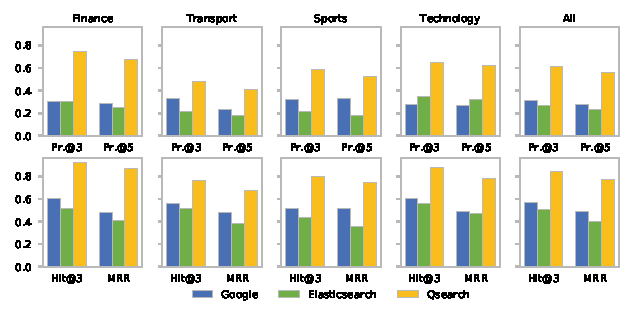
\includegraphics[width= 1\textwidth]{figures/compare.pdf}
	\caption{Comparison of Qsearch against baselines.}
	\label{fig:top-3_comparison}
\end{figure}

Overall, Qsearch performs amazingly well, typically with MRR around 0.7 or better.
The best results are for the 
Finance domain, which has the highest share in the corpus and is most represented in the
Qfact extraction training.
%Finance is the dominating slice of news articles and it covers two most frequent sample categories, Money and %Percentage, in our training dataset. 
%We can also observe that \textit{Precision@k} decreases sharply as \textit{k} increases, together with a high %\textit{MRR} and \textit{Hit} values for our both ranking models, which confirms that relevant entities are ranked higher %by our system than the irrelevant ones. 
\textit{Precision@1} is pretty good, but precision drops substantially when going deeper in the rankings. 
The embedding-based ranking model clearly outperformed the KL-divergence method
by a significant margin.
 
Figure~\ref{fig:top-3_comparison} presents the comparison of Qsearch with the $ced$ ranking model 
against Elasticsearch and Google, showing the metrics \textit{Prec.@3}, \textit{Prec.@5}, \textit{Hit@3} and \textit{MRR}. The results 
clearly indicate that Qsearch outperforms both baselines by a large margin.












